\documentclass[uplatex]{jsarticle}
\usepackage[dvipdfmx]{graphicx}
\title{ソフトウェア設計法2}

\author{101730153 佐治 礼仁 saji.ayahito@h.mbox.nagoya-u.ac.jp}
\date{\today}
\begin{document}
\maketitle
\section{総務省の番号ポータビリティ(MNP)システムを構造化分析し,転入側と転出側の両方について書け}
\subsection{定義した仕様}
総務省の番号ポータビリティ(MNP)システムとは,携帯電話・PHSの利用者が電話会社を変更した場合に,電話番号はそのままで変更後の電話会社のサービスを利用できる制度である.
まず,利用者から移転元事業者に番号ポータビリティの予約を行う.予約が適切に行われたら,移転元事業者からMNP予約番号を受け取る.
利用者は受け取ったMNP予約番号を,移転先事業者に登録して,新規契約申し込みを行う.
移転先事業者は移転元事業者からMNP予約番号等の情報を受け取り,照合した利用者の契約を解除する.
利用者は,移転先との契約に基づいて電話機を受け取る.
\subsection{コンテクストダイアグラム}
コンテクストダイアグラムを図\ref{fig:context-diagram}に記載する.
\begin{figure}[htbp]
  \begin{center}
    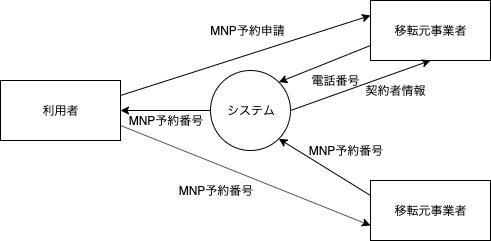
\includegraphics[clip,width=10.0cm]{figures/context-diagram.png}
    \caption{コンテキスト図}
    \label{fig:context-diagram}
  \end{center}
\end{figure}
\subsection{レベル0のデータフローダイアグラム}
データフローダイアグラムを図\ref{fig:dataflow-diagram}に記載する.
\begin{figure}[htbp]
  \begin{center}
    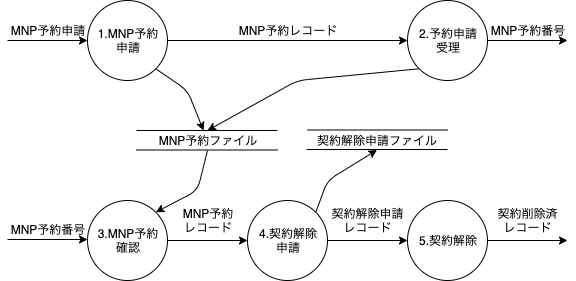
\includegraphics[clip,width=10.0cm]{figures/dataflow-diagram.png}
    \caption{データフロー図}
    \label{fig:dataflow-diagram}
  \end{center}
\end{figure}
\subsection{データディクショナリ}
次のようにデータディクショナリを定義する.

MNP申請予約=電話番号+契約者氏名+契約者住所+契約者年齢

MNP予約レコード=MNP予約番号+電話番号+契約者氏名+契約者住所

\end{document}
